\documentclass[12pt,letterpaper]{article}
\usepackage[utf8]{inputenc}
\usepackage[T1]{fontenc}
\usepackage[activeacute,spanish]{babel}
\usepackage[left=18mm,right=18mm,top=21mm,bottom=21mm,letterpaper]{geometry}%
\usepackage{helvet}
\usepackage{amsmath,amsfonts,amssymb,commath}
\usepackage{graphicx}
\usepackage{color}
\usepackage{xcolor}
\usepackage{verbatim}
\usepackage{tabls}
\usepackage[space]{grffile}
\usepackage{url}
\usepackage{listings}
\usepackage{circuitikz}
\usepackage{siunitx}

\usepackage{matlab-prettifier}

\usepackage{textcomp}
\usepackage{booktabs}
\usepackage[colorlinks=true,urlcolor=blue,linkcolor=black,citecolor=black]{hyperref} 
\usepackage{pdfpages}   %incluir paginas de pdf externo, para los anexos
\usepackage{caption}
\usepackage{subcaption}  
\usepackage{rotating}
\usepackage[section]{placeins}
\usepackage{tikz}

\begin{document}

\title{Laboratorio 2 MATLAB}
\author{Daniel García Vaglio (B42781), Esteban Zamora (B47769), Ariel Fallas (B42481)}
\maketitle

\section{Ejercico 1}
Se hizo primero la simulación con las condiciones iniciales descritas. Para poder resolver el sistema de ecuaciones diferenciales se utilizó el comando ode45. Este comando integra las ecuaciones diferenciales desde un tiempo inicial hasta un tiempo final, para obtener la respuesta respecto al tiempo de las funciones en cuestión. Este es un método de orden intermedio. 

Para resolver el sistema de ecuaciones diferenciales se creó una función en matlab que describe el comportamiento diferencial del sistema, se le llamó odefun. Esta recibe como parámetros un vector de estados, un vector de tiempo, y los parámetros a, b y c. Se utilizó en ode45 para describir las ecuaciones y que este comando se encargue de hacer las integraciones necesarias para encontrar la solución. Se le indica  a ode45 que las variables que debe utilizar son el tiempo y los estados, y que tome los otros parámetros de odefun como constantes. Se presenta el comando (donde t\_sim\_1 es el vector de tiempo, x\_sim\_1 los vectores de estados, tspan es el intervalo de tiempo, y x0 el estado inicial):

\begin{lstlisting}[style=Matlab-editor, basicstyle=\mlttfamily]
    [t_sim_1,x_sim_1] = ode45(@(t_sim_1,x_sim_1) odefun(t_sim_1,x_sim_1,a,b,c), tspan, x0);
\end{lstlisting}

La salida de ode45 son 4 vectores. Uno para el tiempo, y los otros para los estados (los vectores de estados se obtuvieron en forma de matriz, pero se trabajaron por separado, como si fueran vectores). Para encontrar el valor final se revisó la última entrada del vector de estados de la siguiente manera:

%esto es codigo de matla. hay que ponerlo en formato

\begin{lstlisting}[style=Matlab-editor, basicstyle=\mlttfamily]
    valor_final_primera_simulacion=x_sim_1(end,:)
\end{lstlisting}

El resultado obtenido es: $(x_f, y_f, z_f)=$(-1.3972, 0.3190, 5.7522).
Las gráficas solicitadas se presentan en la figura \ref{fig:simulacion1_total}. Para poder graficarlas como se pide en el enunciado, se utilizó el siguiente comando:

\begin{lstlisting}[style=Matlab-editor, basicstyle=\mlttfamily]
    surface([x_sim_1(:,1), x_sim_1(:,1)], [x_sim_1(:,2), x_sim_1(:,2)], [x_sim_1(:,3), x_sim_1(:,3)], [t_sim_1, t_sim_1], 'EdgeColor', 'flat');
\end{lstlisting}

Se hicieron otras 4 simulaciones, la segunda y tercera simulación, son cambiando el parámetro b; la cuarta y quinta son cambiando las condiciones iniciales. En la tabla \ref{table:finales_ejercicio_1}, se presentan los resultados de los valores finales en cada simulación. Las gráficas de la segunda, tercera, cuarta y quinta simulación se presentan en las figuras \ref{fig:simulacion2_total}, \ref{fig:simulacion3_total}, \ref{fig:simulacion4_total}, \ref{fig:simulacion5_total} respectivamente. 

A priori, se puede afirmar que este sistema presenta una alta sensibilidad a los cambios en los parámetros. Note de la tabla \ref{table:finales_ejercicio_1}, que hay grandes cambios en el estado final, con pequeños cambios en los parámetros. Para poder analizar este fenómeno con mayor propiedad, se diseñó un pequeño experimento de simulación. Cómo en las simulaciones propuestas, únicamente varía el parámetro b, entonces se decide hacer un barrido por los valores de b desde 4.85 hasta 8.6 en pasos de 0.05. Estos valores inicial y final son el mínimo valor y máximo de b con los que se hicieron las simulaciones pasadas. El resto de parámetros y el estado inicial, es el mismo que en la primera simulación. Entonces, para cada valor de b se grafica el valor final de los tres estados. El resultado se presenta en la gráfica \ref{fig:sensibilidad}. Es evidente que el estado final varía mucho, con cambios pequeños en la entrada. Entonces se concluye que el sistema es muy sensible.

 




\begin{table}
\caption{Valores finales de cada simulación}
\label{table:finales_ejercicio_1}
\centering
\begin{tabular}{| c | c  c  c|}
  \hline
 Simulación & b   & $x_0$   & $x_f$   \\
 \hline
 Primera    & 4.85&( 2.3, -1.3,  10) &( -1.3972, 0.3190, 5.7522) \\
 Segunda    & 8.5& ( 2.3, -1.3,  10) &( 2.8602,  1.4443, 2.7291) \\
 Tercera    & 8.6& ( 2.3, -1.3,  10) &( 44.4532, 3.3235, 17.0307)\\
 Cuarta     & 4.85&(-2.3,  1.3, -10) &( 8.0713,  0.4780, 8.3260)\\
 Quinta     & 4.85&(-0.1, -1,    -1) &( 24.0736, 6.4495, 12.8533)\\
 \hline

\end{tabular}
\end{table}


%Primera simulacion ···········································································································································
\begin{figure}
	\centering
	\begin{subfigure}[t]{0.36\textwidth}
		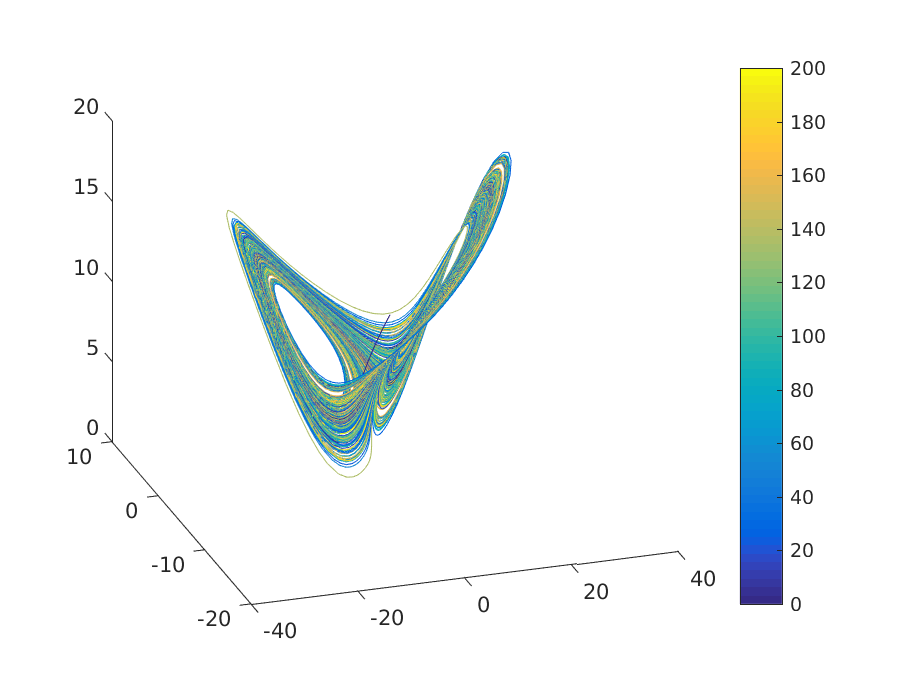
\includegraphics[width=\textwidth]{pictures/primera_simulacion}
		\caption{Resultado para primer caso de condiciones ininciales}
		\label{fig:simulacion1}
	\end{subfigure}
	\begin{subfigure}[t]{0.36\textwidth}
		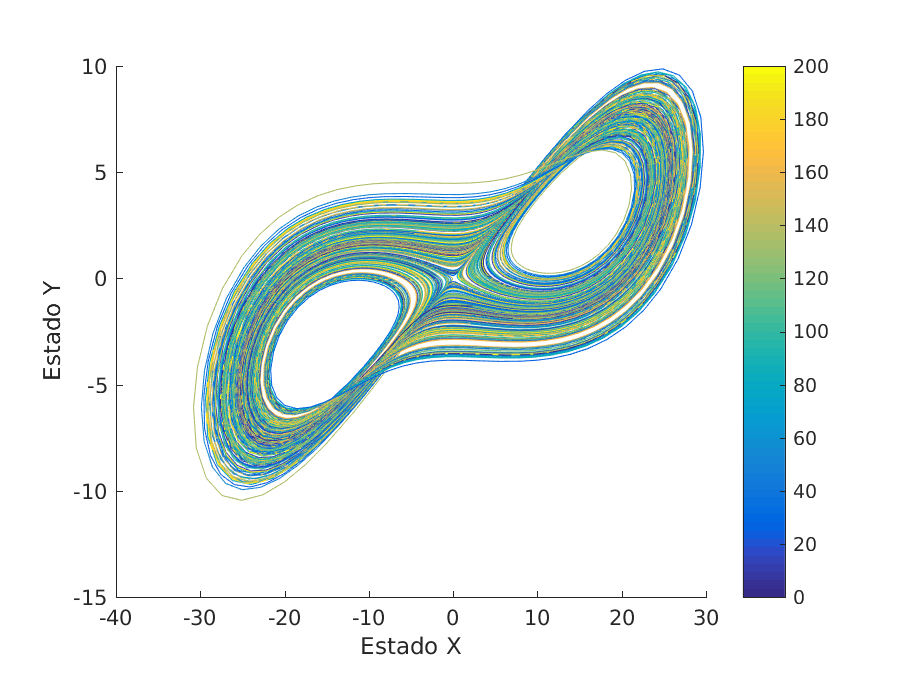
\includegraphics[width=\textwidth]{pictures/primera_simulacion_xy}
		\caption{Vista XY de la primera simulación}
		\label{fig:simulacion1xy}
	\end{subfigure}
        \vfill
        \begin{subfigure}[b]{0.36\textwidth}
		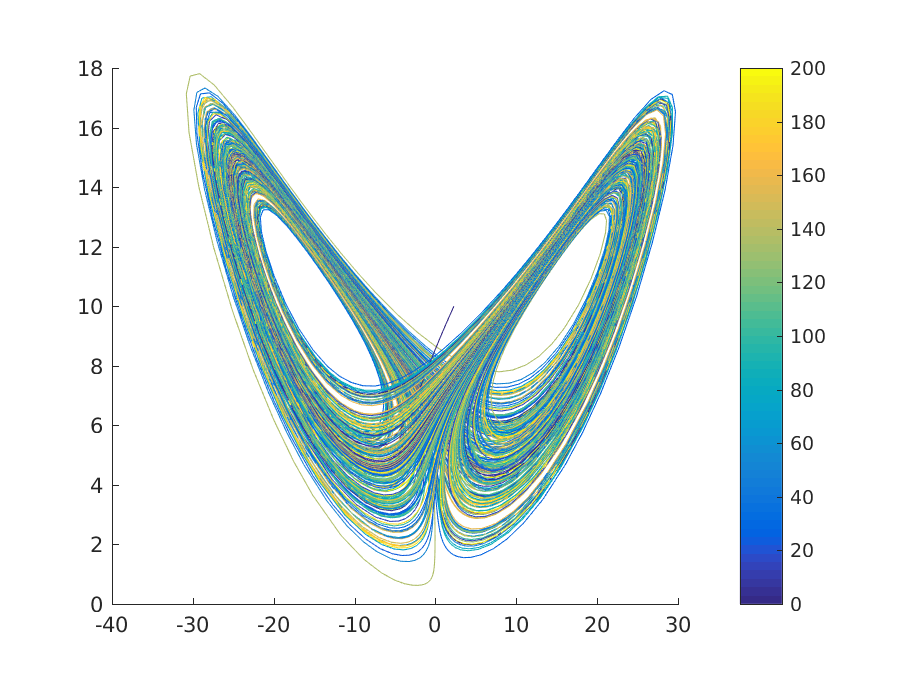
\includegraphics[width=\textwidth]{pictures/primera_simulacion_xz}
		\caption{Vista XZ de la primera simulación}
		\label{fig:simulacion1xz}
	\end{subfigure}
        \begin{subfigure}[b]{0.36\textwidth}
		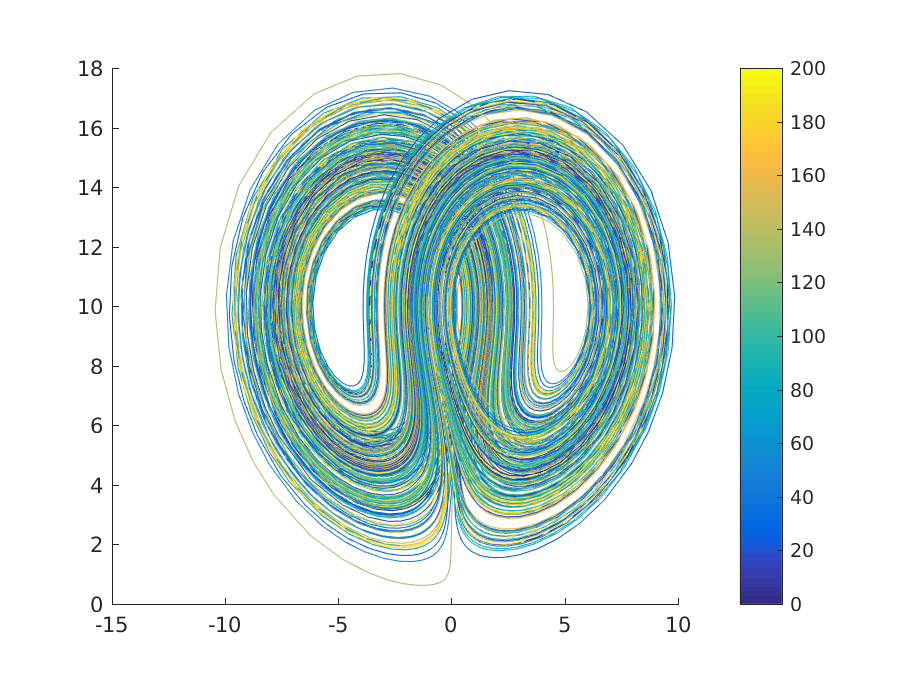
\includegraphics[width=\textwidth]{pictures/primera_simulacion_yz}
		\caption{Vista YZ de la primera simulación}
		\label{fig:simulacion1yz}
	\end{subfigure}
	\caption{Primera simulación gráfica de los estados. En los ejes se tienen los estados y el tiempo se denota con el cambio de color}
	\label{fig:simulacion1_total}
\end{figure}

%segunda simulacion ···········································································································································
\begin{figure}
	\centering
	\begin{subfigure}[t]{0.36\textwidth}
		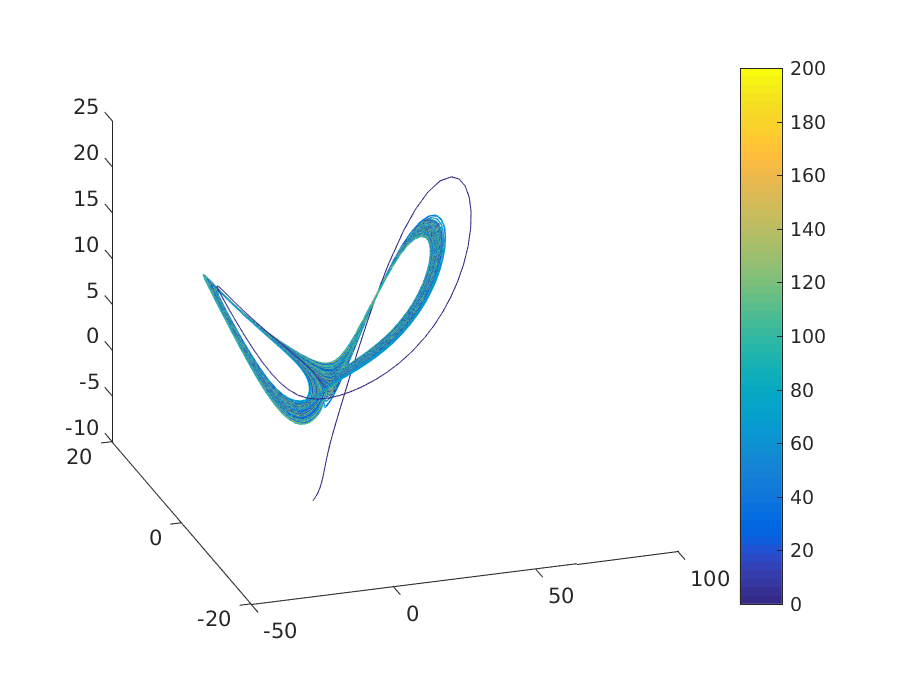
\includegraphics[width=\textwidth]{pictures/segunda_simulacion}
		\caption{Resultado para primer caso de condiciones ininciales}
		\label{fig:simulacion2}
	\end{subfigure}
	\begin{subfigure}[t]{0.36\textwidth}
		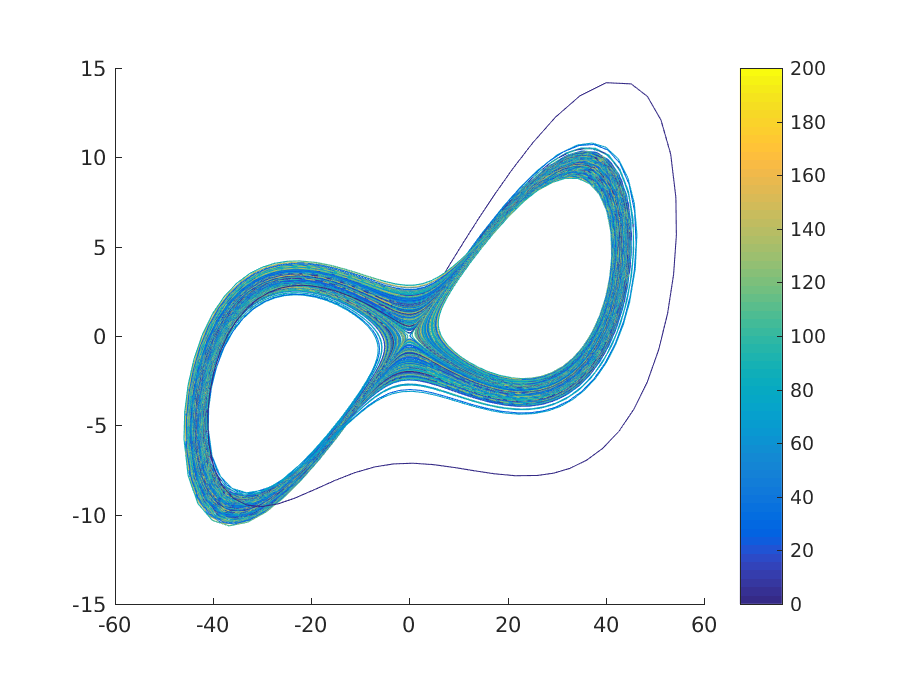
\includegraphics[width=\textwidth]{pictures/segunda_simulacion_xy}
		\caption{Vista XY de la segunda simulación}
		\label{fig:simulacion2xy}
	\end{subfigure}
        \vfill
        \begin{subfigure}[b]{0.36\textwidth}
		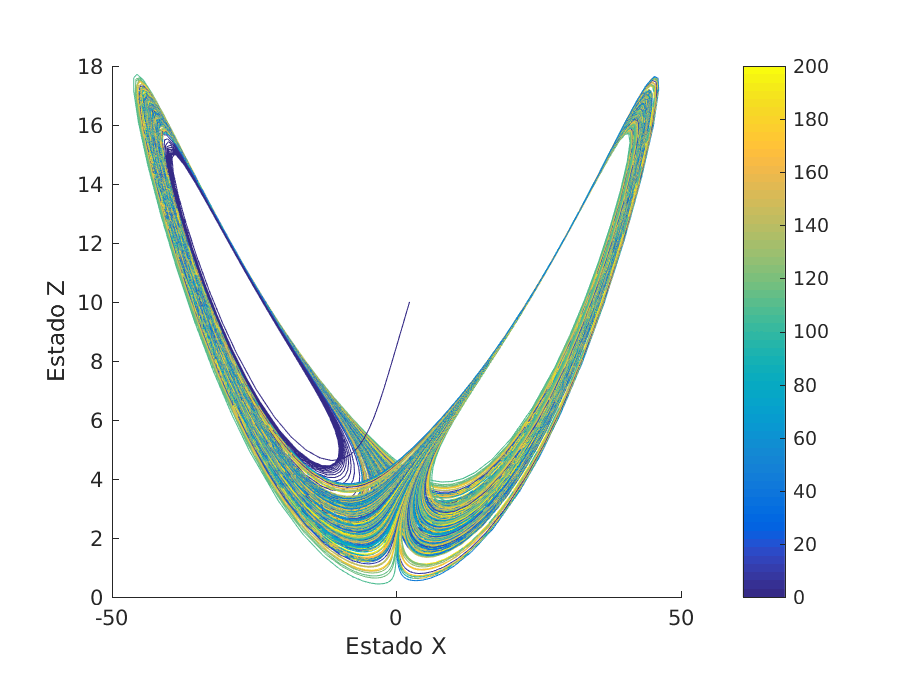
\includegraphics[width=\textwidth]{pictures/segunda_simulacion_xz}
		\caption{Vista XZ de la segunda simulación}
		\label{fig:simulacion2xz}
	\end{subfigure}
        \begin{subfigure}[b]{0.36\textwidth}
		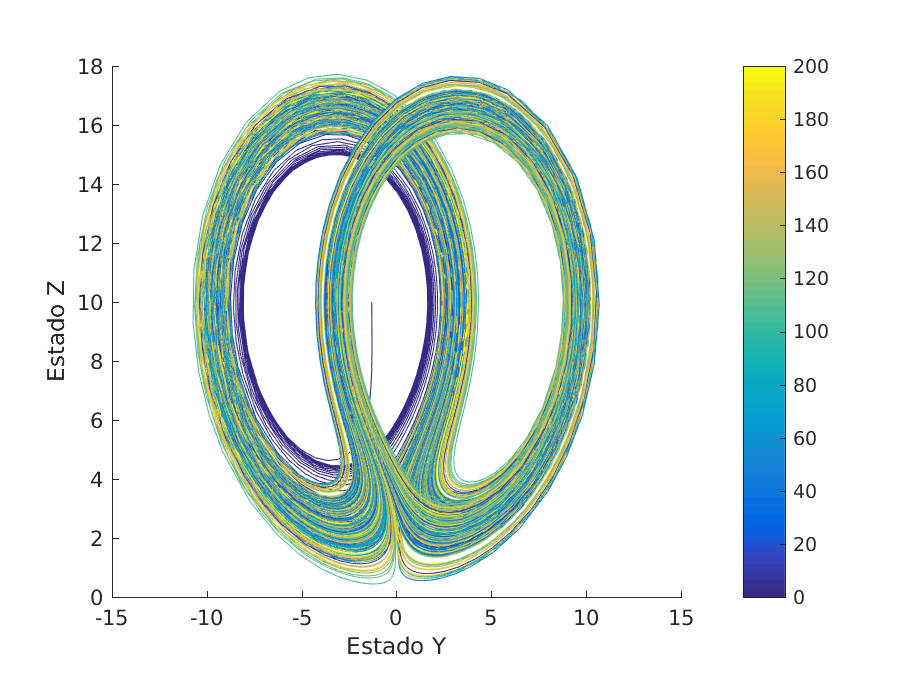
\includegraphics[width=\textwidth]{pictures/segunda_simulacion_yz}
		\caption{Vista YZ de la segunda simulación}
		\label{fig:simulacion2yz}
	\end{subfigure}
	\caption{Segunda simulación gráfica de los estados. En los ejes se tienen los estados y el tiempo se denota con el cambio de color}
	\label{fig:simulacion2_total}
\end{figure}

%Tercera simulacion ···········································································································································

\begin{figure}
	\centering
	\begin{subfigure}[t]{0.36\textwidth}
		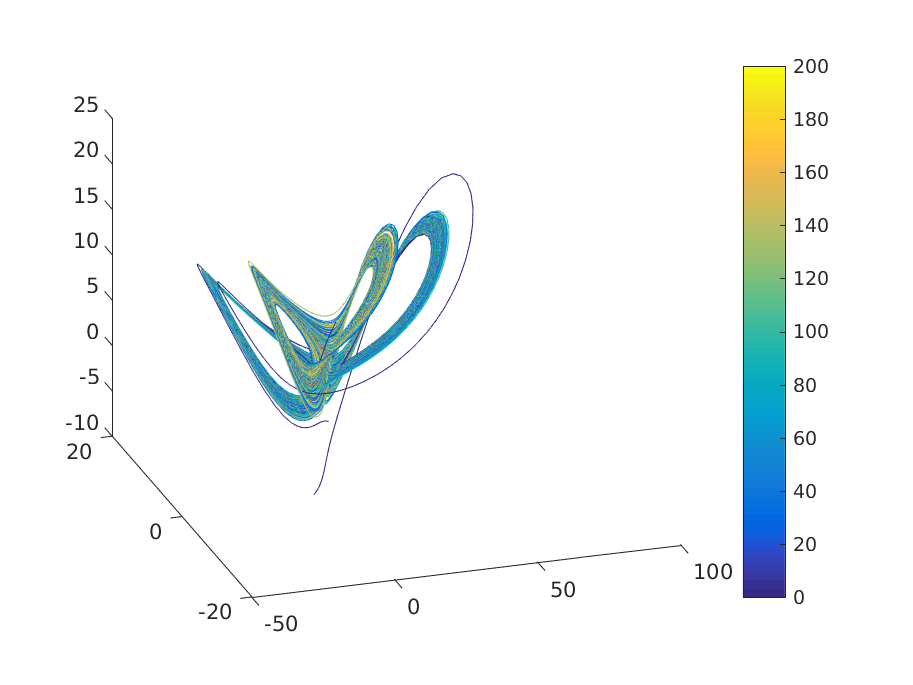
\includegraphics[width=\textwidth]{pictures/tercera_simulacion}
		\caption{Resultado para primer caso de condiciones ininciales}
		\label{fig:simulacion3}
	\end{subfigure}
	\begin{subfigure}[t]{0.36\textwidth}
		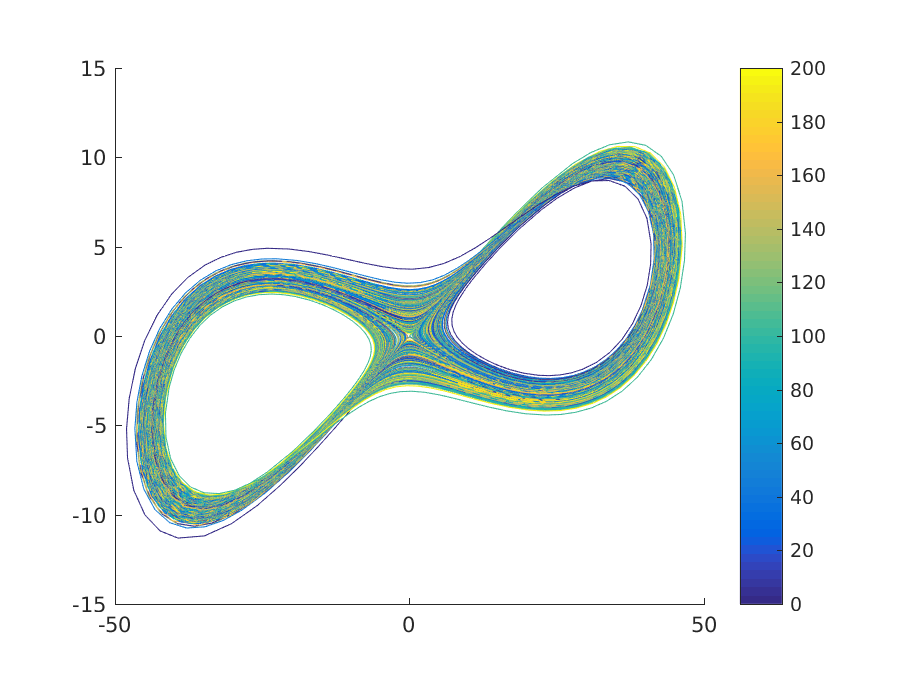
\includegraphics[width=\textwidth]{pictures/tercera_simulacion_xy}
		\caption{Vista XY de la tercera simulación}
		\label{fig:simulacion3xy}
	\end{subfigure}
        \vfill
        \begin{subfigure}[b]{0.36\textwidth}
		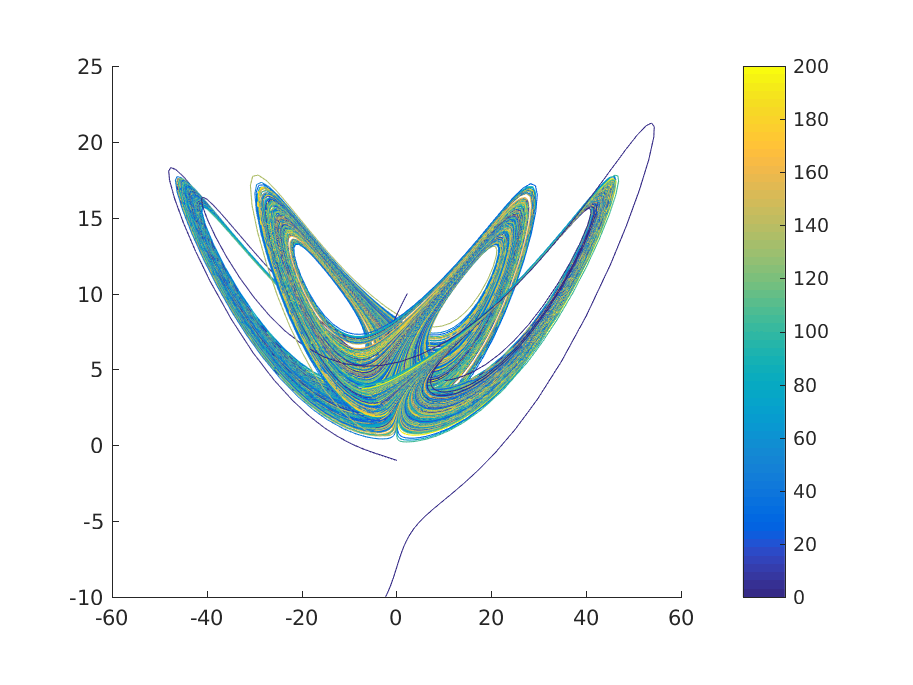
\includegraphics[width=\textwidth]{pictures/tercera_simulacion_xz}
		\caption{Vista XZ de la tercera simulación}
		\label{fig:simulacion3xz}
	\end{subfigure}
        \begin{subfigure}[b]{0.36\textwidth}
		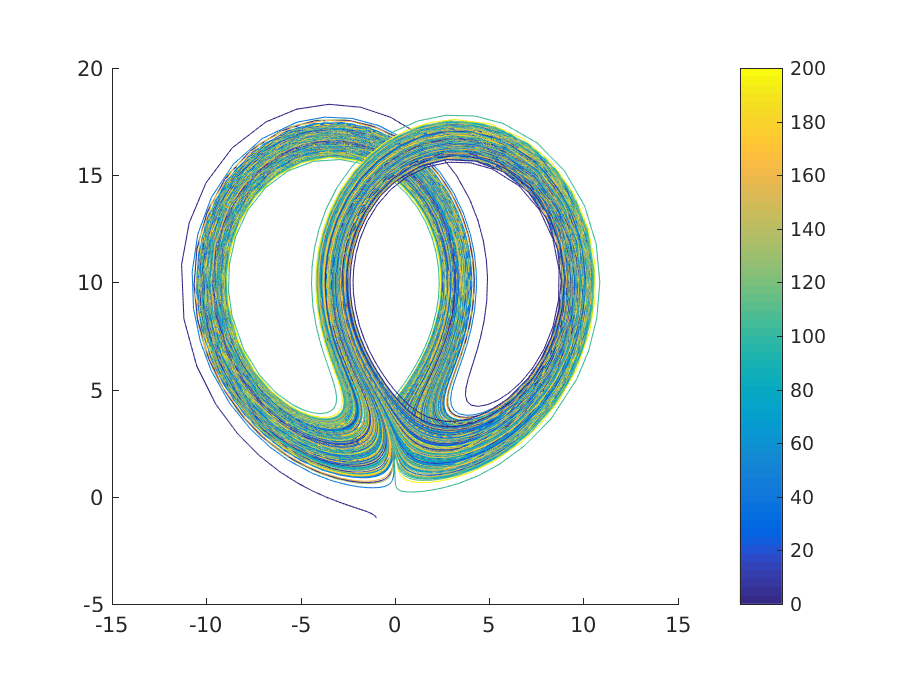
\includegraphics[width=\textwidth]{pictures/tercera_simulacion_yz}
		\caption{Vista YZ de la tercera simulación}
		\label{fig:simulacion3yz}
	\end{subfigure}
	\caption{Tercera simulación gráfica de los estados. En los ejes se tienen los estados y el tiempo se denota con el cambio de color}
	\label{fig:simulacion3_total}
\end{figure}

%cuarta simulacion·····································································

\begin{figure}
	\centering
	\begin{subfigure}[t]{0.36\textwidth}
		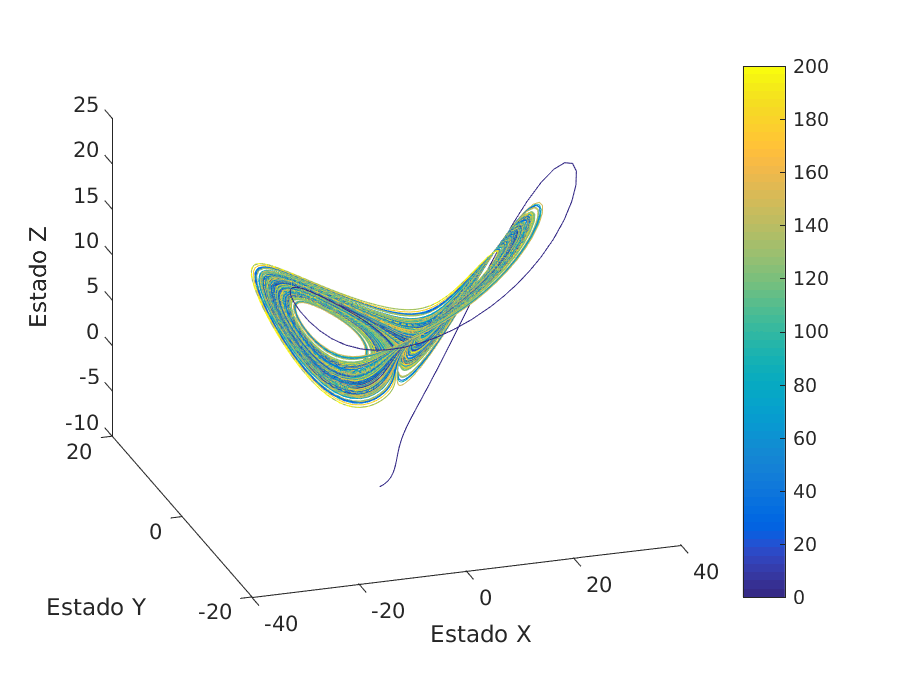
\includegraphics[width=\textwidth]{pictures/cuarta_simulacion}
		\caption{Resultado para primer caso de condiciones ininciales}
		\label{fig:simulacion4}
	\end{subfigure}
	\begin{subfigure}[t]{0.36\textwidth}
		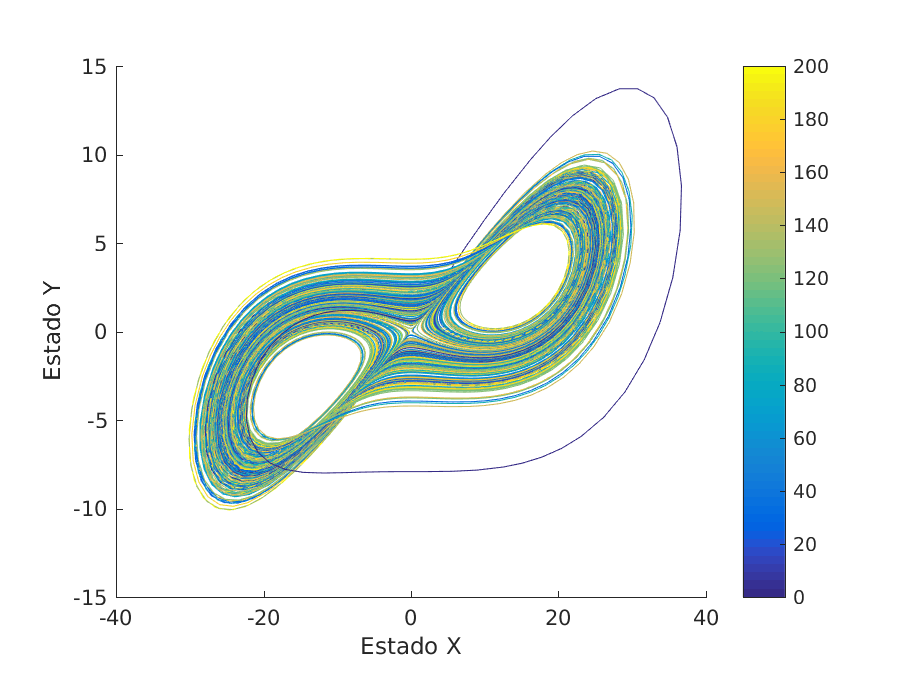
\includegraphics[width=\textwidth]{pictures/cuarta_simulacion_xy}
		\caption{Vista XY de la cuarta simulación}
		\label{fig:simulacion4xy}
	\end{subfigure}
        \vfill
        \begin{subfigure}[b]{0.36\textwidth}
		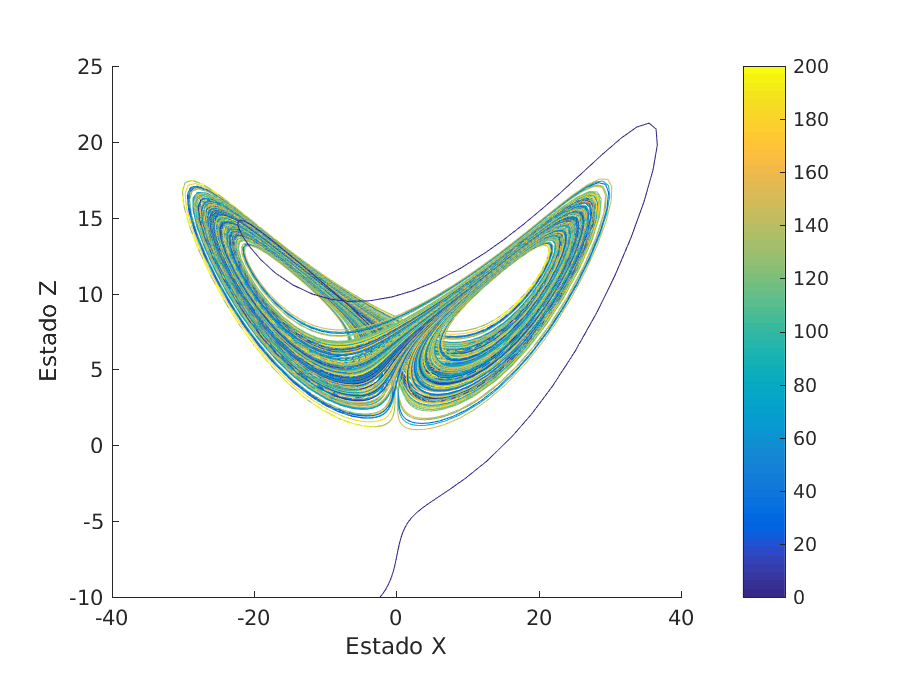
\includegraphics[width=\textwidth]{pictures/cuarta_simulacion_xz}
		\caption{Vista XZ de la cuarta simulación}
		\label{fig:simulacion4xz}
	\end{subfigure}
        \begin{subfigure}[b]{0.36\textwidth}
		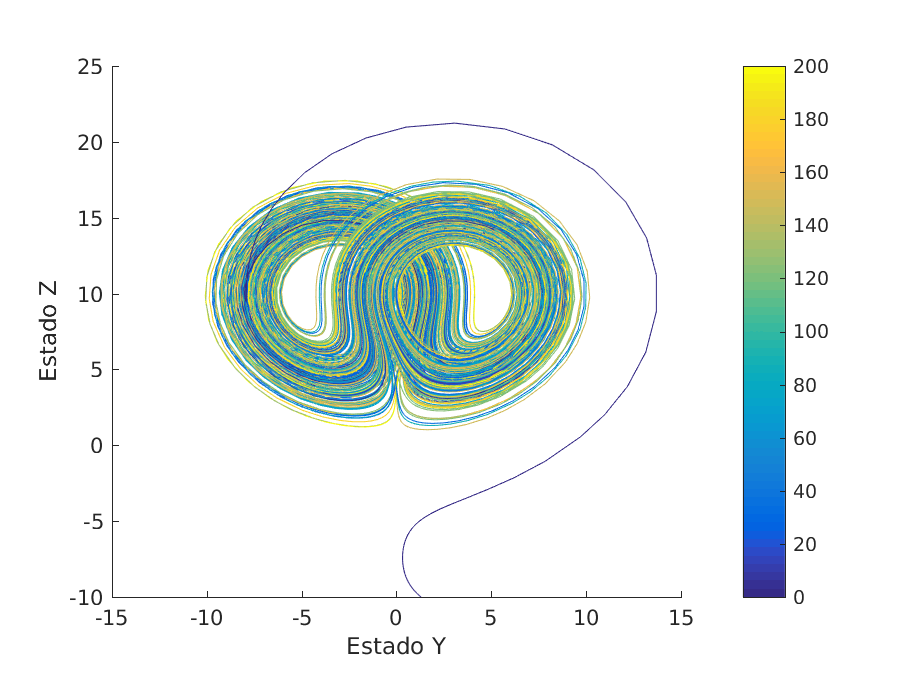
\includegraphics[width=\textwidth]{pictures/cuarta_simulacion_yz}
		\caption{Vista YZ de la cuarta simulación}
		\label{fig:simulacion4yz}
	\end{subfigure}
	\caption{Cuarta simulación gráfica de los estados. En los ejes se tienen los estados y el tiempo se denota con el cambio de color}
	\label{fig:simulacion4_total}
\end{figure}

%quinta simulacion························································
\begin{figure}
	\centering
	\begin{subfigure}[t]{0.36\textwidth}
		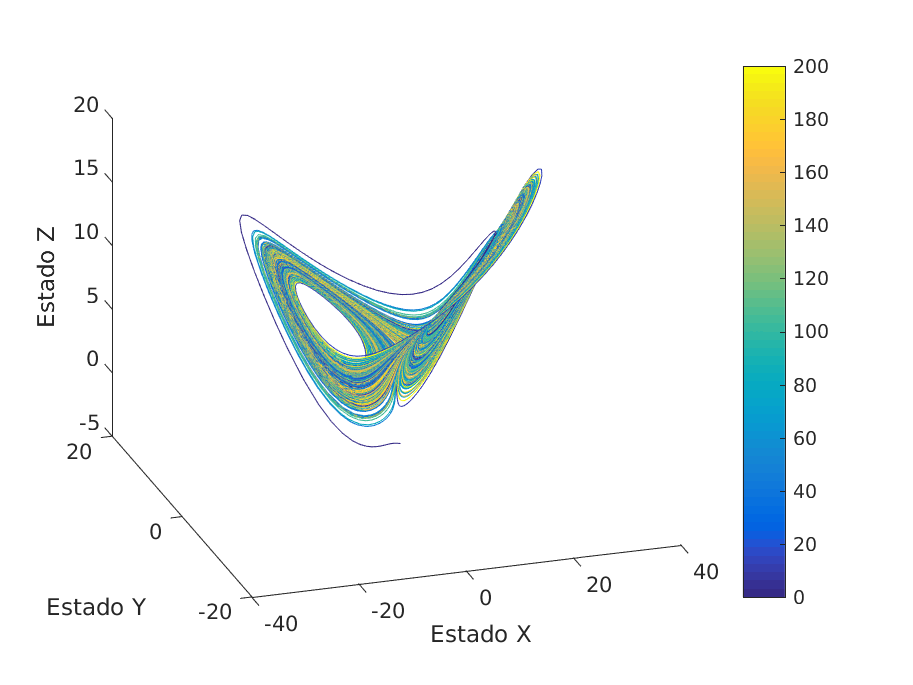
\includegraphics[width=\textwidth]{pictures/quinta_simulacion}
		\caption{Resultado para primer caso de condiciones ininciales}
		\label{fig:simulacion5}
	\end{subfigure}
	\begin{subfigure}[t]{0.36\textwidth}
		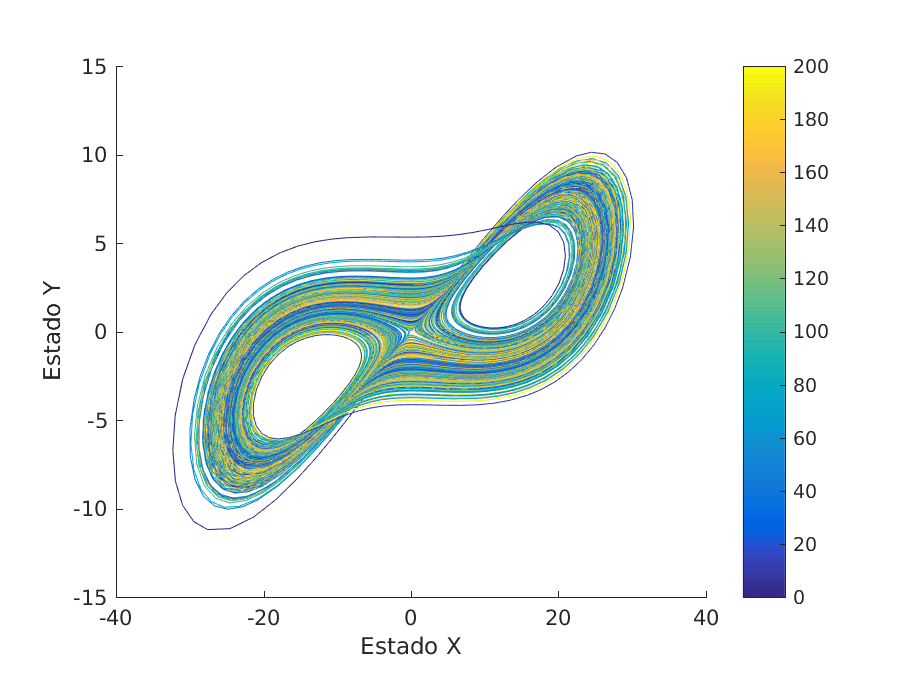
\includegraphics[width=\textwidth]{pictures/quinta_simulacion_xy}
		\caption{Vista XY de la quinta simulación}
		\label{fig:simulacion5xy}
	\end{subfigure}
        \vfill
        \begin{subfigure}[b]{0.36\textwidth}
		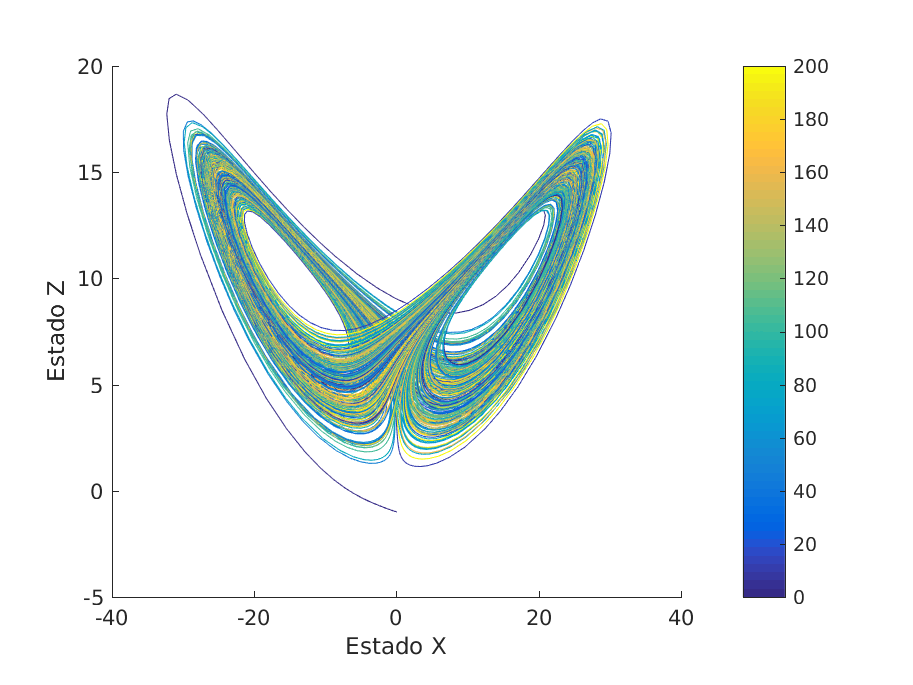
\includegraphics[width=\textwidth]{pictures/quinta_simulacion_xz}
		\caption{Vista XZ de la quinta simulación}
		\label{fig:simulacion5xz}
	\end{subfigure}
        \begin{subfigure}[b]{0.36\textwidth}
		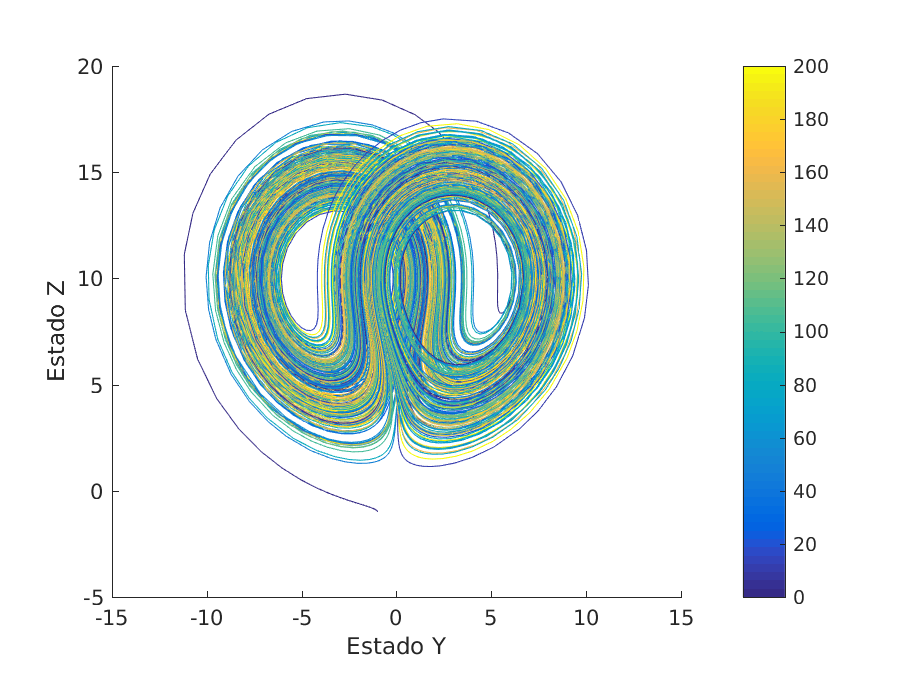
\includegraphics[width=\textwidth]{pictures/quinta_simulacion_yz}
		\caption{Vista YZ de la quinta simulación}
		\label{fig:simulacion5yz}
	\end{subfigure}
	\caption{Quinta simulación gráfica de los estados. En los ejes se tienen los estados y el tiempo se denota con el cambio de color}
	\label{fig:simulacion5_total}
\end{figure}
%Comparacion de los estados de las distintas simulaciones respecto al tiempo.···················································································

\begin{figure}
	\centering
	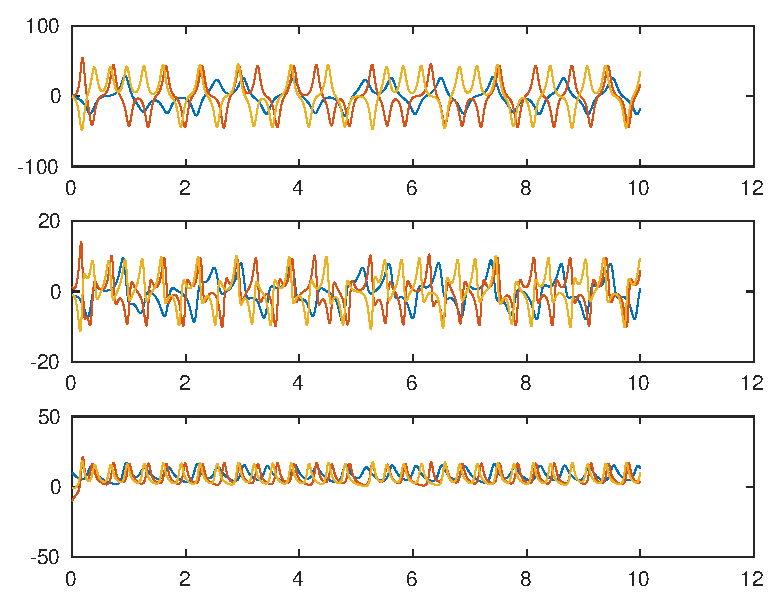
\includegraphics[width=0.8\textwidth]{pictures/comparacion}
	\caption{Comparación de los estados de las distintas simulaciones respecto al tiempo. Se presentan en rojo, verde, azul, magenta, y cían respectivamente cada simulación.}
	\label{fig:comparacion}
\end{figure}

%Sensibilidad respecto a los parámetros···················································································

\begin{figure}
	\centering
	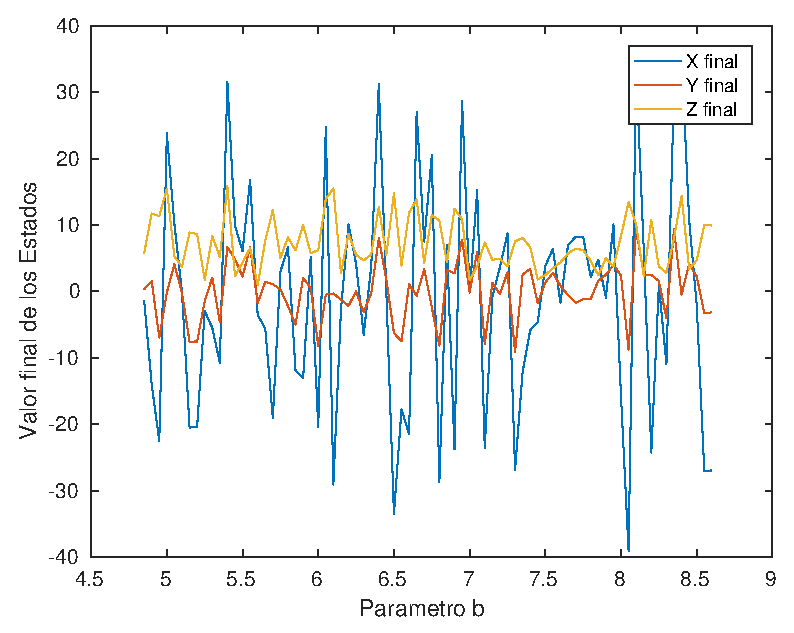
\includegraphics[width=0.8\textwidth]{pictures/sensibilidad}
	\caption{Valor final de cada estado, dependiendo del valor de b}
	\label{fig:sensibilidad}
\end{figure}

\subsection{Código del script principal}
Del script principal, solo se agrega la parte inicial. Ya que el resto del código es una repetición de lo primero, pero para las otras simulaciones.
\lstinputlisting[style=Matlab-editor, basicstyle=\mlttfamily, firstline=6, lastline=45]{Ejercicio1.m}

Se agrega también el código para hacer la gráfica comparativa de todos los estados en 10 segundos.

\lstinputlisting[style=Matlab-editor, basicstyle=\mlttfamily, firstline=161, lastline=197]{Ejercicio1.m}
\subsection{Código de odefun()}
\lstinputlisting[style=Matlab-editor, basicstyle=\mlttfamily, firstline=5]{odefun.m}
\subsection{Código de sensibilidad}
Este código es parte del script principal. Pero como no es parte de lo que se pide explícitamente, entonces se agrega por aparte en este documento.
 
\lstinputlisting[style=Matlab-editor, basicstyle=\mlttfamily, firstline=201]{Ejercicio1.m}




\section{Ejercicio 2}


\subsection{Código de ejercicio 2}

\section{Ejercicio 3}

\subsection{S-Function para el modelo del cohete}

%Condiciones iniciales
\begin{lstlisting}[style=Matlab-editor, basicstyle=\mlttfamily]
  function InitConditions(block) %Se inicializan los estados
    % Altura inicial
    block.ContStates.Data(1) = 0;
    % Velocidad inicial
    block.ContStates.Data(2) = 0;
    % Masa inicial
    block.ContStates.Data(3) = block.DialogPrm(7).Data;
\end{lstlisting}

%Salidas
\begin{lstlisting}[style=Matlab-editor, basicstyle=\mlttfamily]
  function Outputs(block) % Se calculan las salidas
    h = block.ContStates.Data(1);
    v = block.ContStates.Data(2);

    % Altura mayor o igual a 0
    if (h < 0)
      block.OutputPort(1).Data = 0;
      block.OutputPort(2).Data = 0;
    else
      block.OutputPort(1).Data = h;
      block.OutputPort(2).Data = v;
    end
\end{lstlisting}

%Derivadas
\begin{lstlisting}[style=Matlab-editor, basicstyle=\mlttfamily]
  function Derivatives(block) % Se calculan las derivadas
    % Estados
    h = block.ContStates.Data(1);
    v = block.ContStates.Data(2);
    mp = block.ContStates.Data(3);

    % Parametros
    ms = block.DialogPrm(1).Data;
    g = block.DialogPrm(2).Data;
    rho = block.DialogPrm(3).Data;
    A = pi*(block.DialogPrm(4).Data)^2;
    ve = block.DialogPrm(5).Data;
    Cd = block.DialogPrm(6).Data;

    % Masa del combustible mayor a 0
    if mp > 0
      up = block.InputPort(1).Data;
    else
      up = 0;
      block.ContStates.Data(3) = 0;
      mp = block.ContStates.Data(3);
    end

    % Derivada h
    block.Derivatives.Data(1) = v;
    % Derivada v
    block.Derivatives.Data(2) = (-(ms+mp)*g + up*ve -(1/2)*rho*v*abs(v)*A*Cd)/(ms+mp);
    % Derivada mp
    block.Derivatives.Data(3) = -up;     
\end{lstlisting}



\subsection{Simulación del movimiento del cohete}


\begin{figure}[ht!]
  \centering
  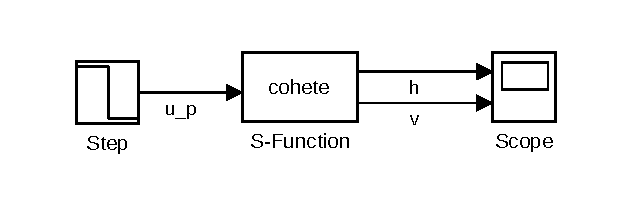
\includegraphics[width=0.5\linewidth]{pictures/Ejercicio3/simulink_cohete.eps}
  \caption{Diagrama de bloques en Simulink}
\end{figure}



\begin{figure}[ht!]
  \centering
  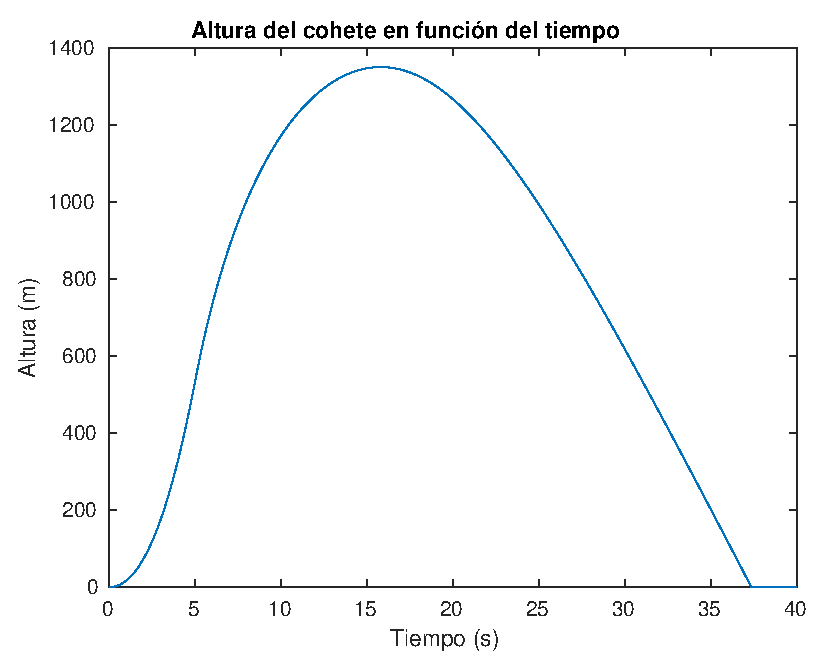
\includegraphics[width=0.5\linewidth]{pictures/Ejercicio3/altura_cohete_vs_tiempo.eps}
  \caption{Gráfica de la altura del cohete con respecto al tiempo}
  \label{fig:alt_cohete}
\end{figure}



\begin{figure}[ht!]
  \centering
  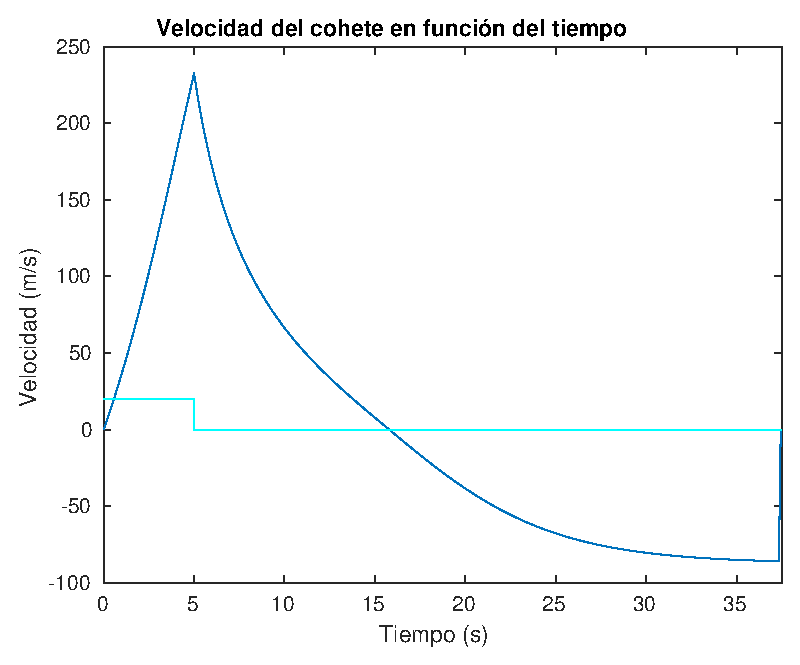
\includegraphics[width=0.5\linewidth]{pictures/Ejercicio3/velocidad_cohete_vs_tiempo.eps}
  \caption{Gráfica de la velocidad del cohete con respecto al tiempo}
\end{figure}







\end{document}
